\section{Method}
\label{sec:method}

The review aspect extraction problem aims to extract or infer $K$ noun 
words from user review texts,
each word should represent a distinct aspect or feature of a type of product or service. 
Here $K$ is an constant parameter for the problem. 
In unsupervised models for aspect extraction, 
the set of reviews and the number of aspects are the only inputs.
Note that in this definition we don't use cross-domain information, 
that is, for one product type we only use the reviews of that domain.
This allows us to apply the model to any domain with ease.

The framework of our method is shown in \figref{fig:framework}, 
it consists of 5 steps. 
In the following we will explain the motivation and the details of each of
the five steps.

\begin{figure}[th]
\centering
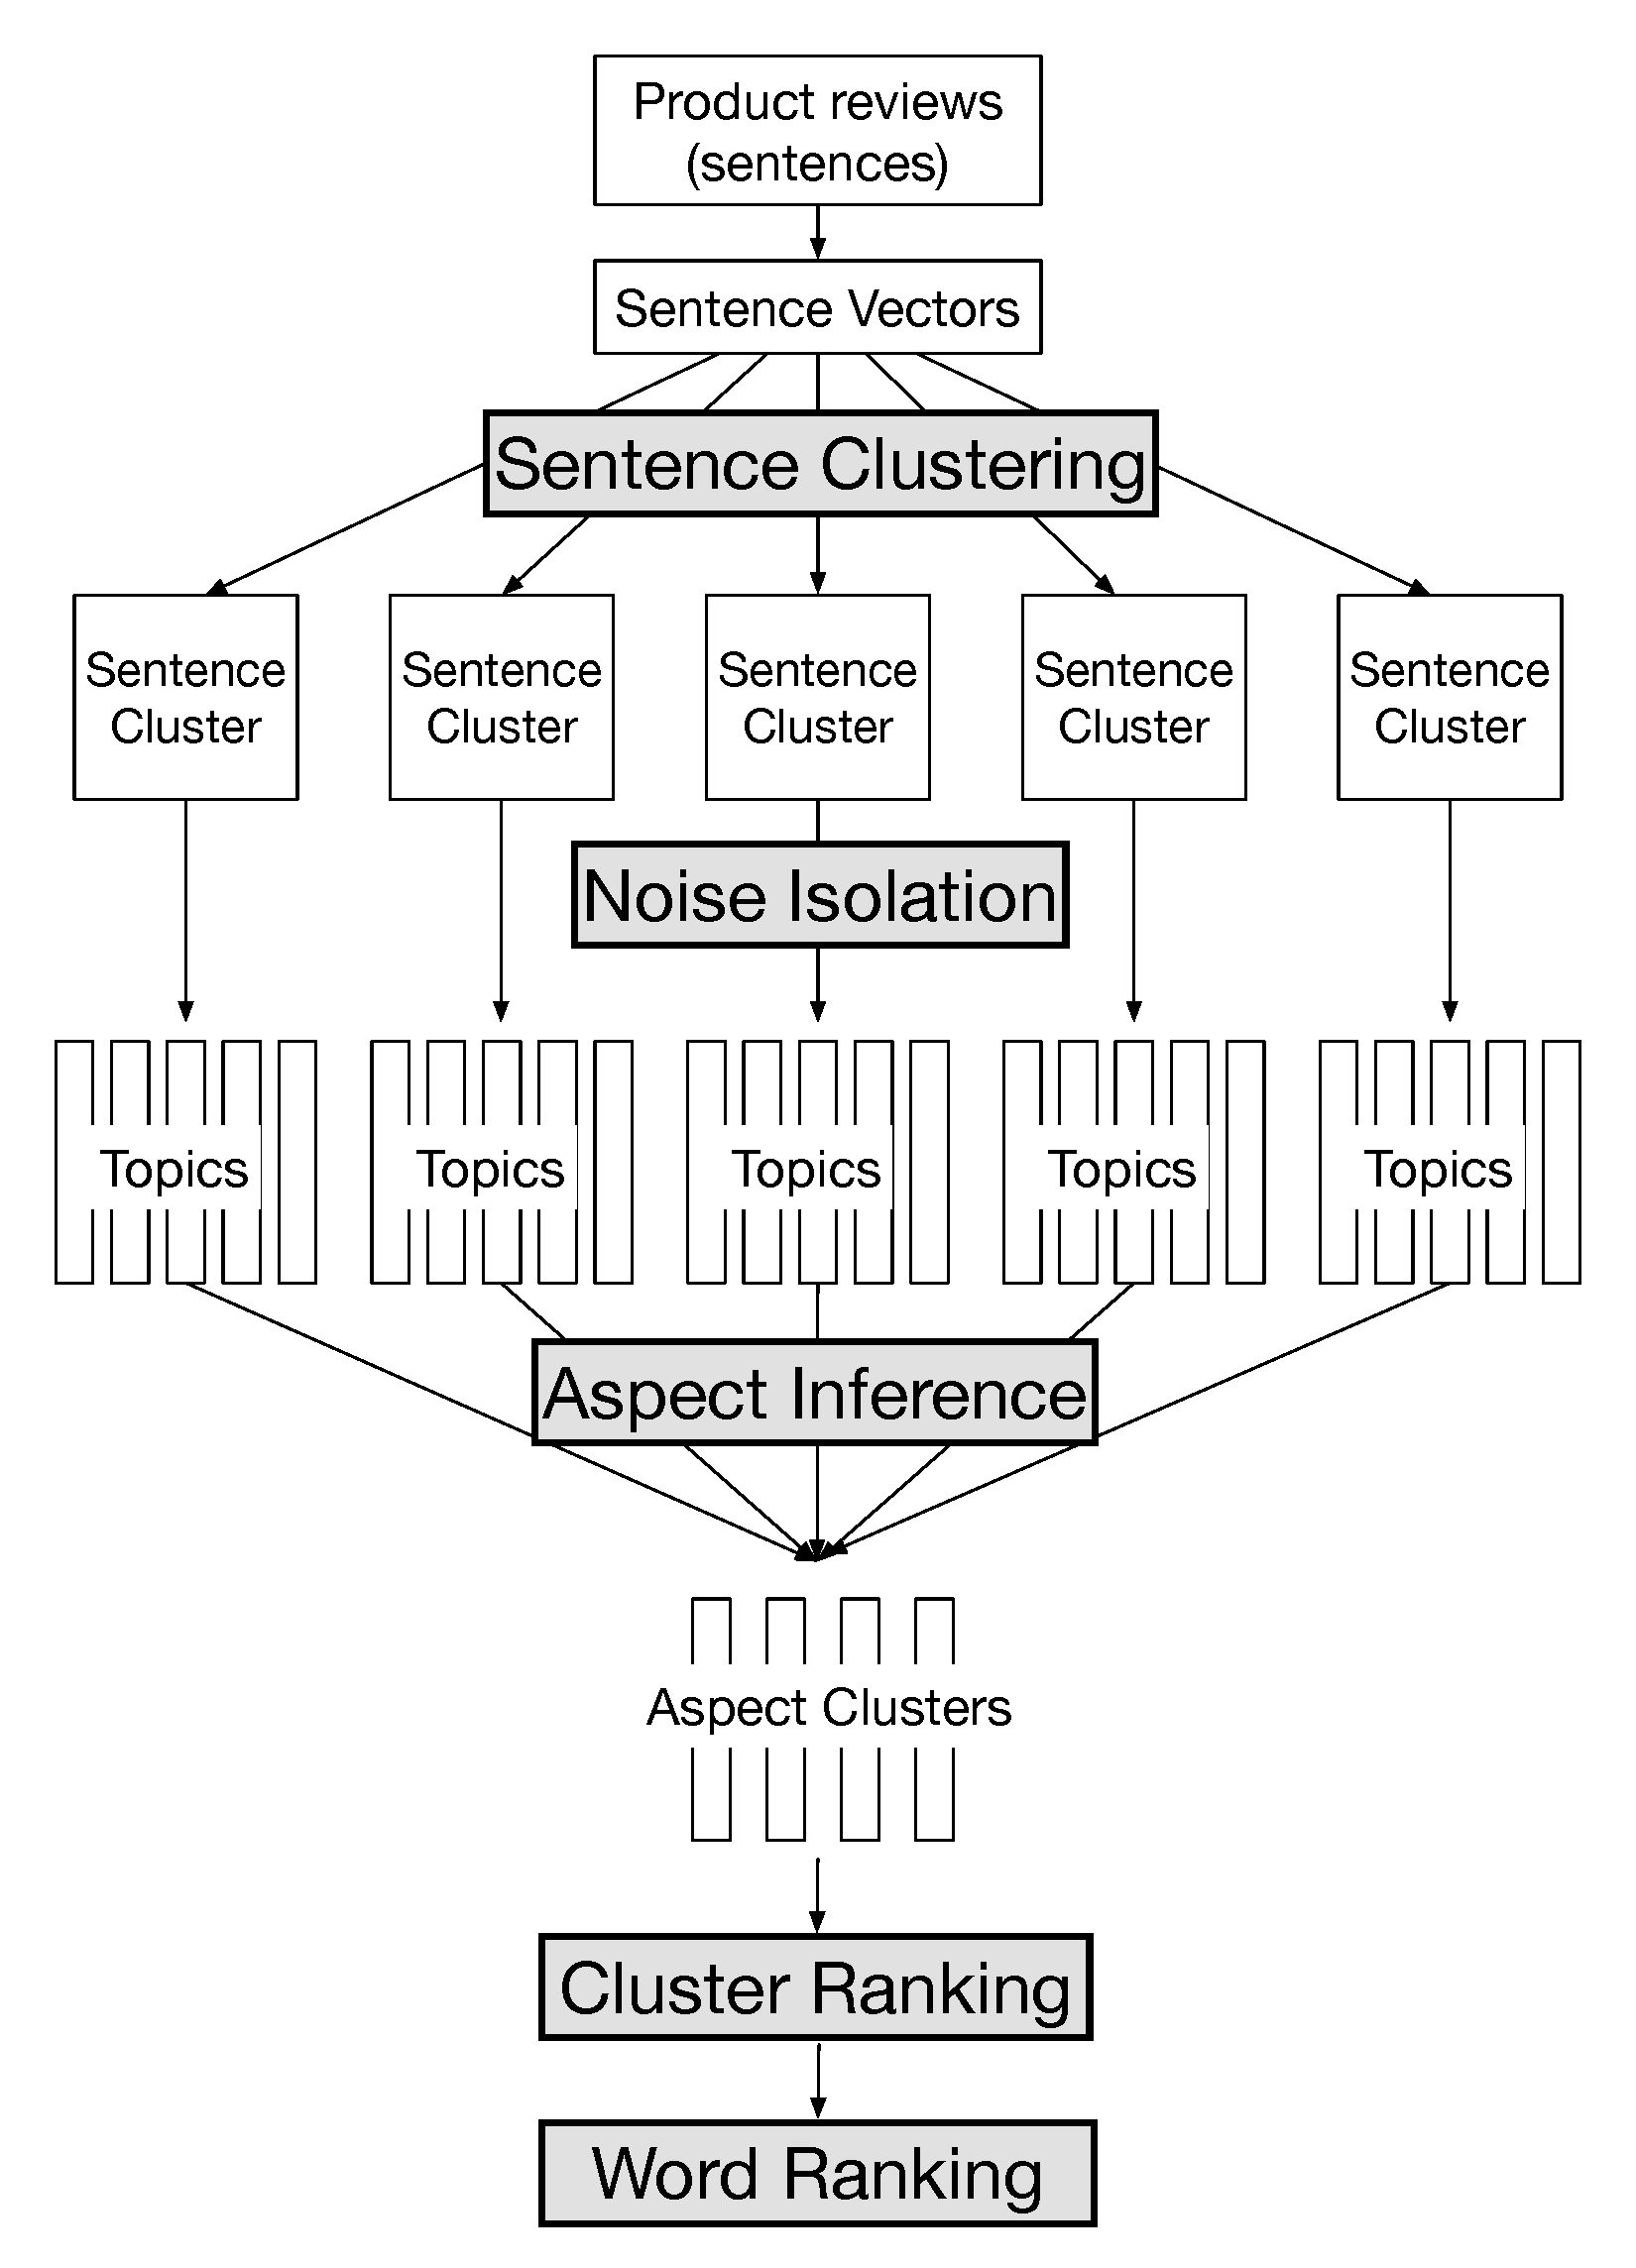
\includegraphics[width=0.9\columnwidth]{figures/framework}
\caption{Our framework.}
\label{fig:framework}
\end{figure}

\subsection{Sentence Clustering}

One important feature of user reviews is that many topics are 
compressed into a short paragraph, where each topic corresponds to 
a potential aspect of the product. 
A typical hotel review extracted from \figref{fig:tripadvisor} 
is shown as follows:

\begin{quote}
Pool is small and only 4 ft but refreshing. Hot tub also there. Staff were super friendly each day. Room was nothing special but clean and comfy. Lots of restaurants and bars nearby. Breakfast was great and despite being a busy weekend there was always a big selection available.
\end{quote}
%we convert each sentence in the reviews into a vector representation 
%and cluster them in to $N$ clusters of semantically similar sentences.

In user reviews, topics can shift very quickly.
Sentences that are close to each other may refer to 
completely different aspects about the product. Also,
sentences about the same aspect may not appear in the review consecutively. 
The existence of such fine-grained semantic shifts in user reviews 
makes it difficult to apply the the bag-of-word abstraction 
of normal topic model on reviews.
Therefore we propose to work on the sentence level instead 
of the document level, and it would be helpful if we can divide the 
reviews into topic-oriented segments.

Driven by this observation, in our method the first step is 
sentence clustering.  
For this purpose, we represent each 
sentence in a low-dimensional vector space.
Instead of using simplistic methods like bag-of-word vector, 
we leverage a recent development of neural network in natural 
language processing, the distributed representation.
In a distributed representation, words and sentences are 
converted into real-valued vectors.
The distance of the vectors in the vector space will capture the 
semantic similarity of the words or sentences.

In this work we train such vector representations on review sentences using paragraph vector (PV) model \cite{le2014distributed}.
We run a k-means clustering on the sentence vectors and generate 
$N$ sentence clusters. We then collect the sentences from the same review 
that are clustered together to form smaller pieces of reviews. 
Each review document is divided into several shorter documents, each belonging
to one of the $N$ clusters. As a result, we obtain $N$ clusters of shorter documents. 

\TODO { 
Use the sentence cluster of the N*M topics as the separation to be evaluated, calculate the  ARI score 
between the initial separation and the groundtruth to show the necessity of the noise isolation step.}

\TODO { 
Propose perplex or purity of topics to delete some mixed topics ? 
Propose an idea to isolate the noisy topics, the intuition is that: 1) some topics mixed serveral other pure topics 
Maybe this is not a big problem since it still contains some useful information. After clustered with some relevant 
topics, it will have a positive effect on the final cluster representation.
2) some topics does discuss a feature but does not in the groundtruth, in the other words, it is not so important to be rating. 
Sometimes the feature may be too specific, then we can use information content to measure this. 
Somtimes the feature is not relevant to the service or product, it just tells us the background or story behind the service or product.
In this situation, such topics' subjectivities are often very weak. 
Maybe we can also measure the subjectivity of the topics. 
3) Another information is that each topic $t$ has a prior $p(t)$, which measures the probability of the topic appears. 
We can also leverage this to measure the topic. }

\subsection{Noise Isolation}

%To isolate the noises that exist in the sentence cluster,
%for each sentence cluster we further generate $M$ 
%topics, resulting in $N\times M$ different word distributions in total.

The first step, sentence clustering, we might include noise and the sentences 
within a cluster might not all be about the same aspect. 
The reason is due to the common occurrences of sentences such as the following
in the reviews (taken from TripAdvisor):

\begin{quote}
The room was clean, the staff were friendly, and I would say the price is very reasonable given the proximity to business and leisure destinations around downtown.
\end{quote}

\begin{quote}
There is a restaurant just 5 min walk away with nice italian food, pizza was great.
\end{quote}

In the first sentence multiple aspects are mentioned; in the second sentence, the only aspect is location however lexically it seems to be talking about food.
With these complicated structures within, 
it is difficult for  PV to correctly determine the aspects 
in these sentences. The result is overlaps between clusters about 
different aspects and noises within each cluster.
To isolate the noises and resolve such overlap between short review pieces, 
we apply Biterm Topic Model (BTM) \cite{cheng2014btm} topic modeling within each sentence cluster 
and generating $M$ smaller topics. 
This will give us in total $N\times M$ topics, or, word distributions. 
\tabref{table:overlap} shows an example of topics inferred from three
sentence clusters from hotel reviews and illustrates the overlap problem.
In this example, five topics were extracted from each sentence cluster, 
and each row is one topic. It can be seen that the aspects for the 
three clusters should be {\em room}, {\em location} and {\em price} 
respectively.
However, topics shown in boldface font obviously belong to 
other clusters.  Especially, the last topic of the third cluster 
appears to be an overlap of more than two clusters.
The noise isolation step effectively separates the noisy topics from other
topics semantically corehent within a sentence cluster.

\begin{table}[th]
\centering
\caption{Topics extracted from three sentence clusters of hotel review.}
\label{table:overlap}
\begin{tabular}{|c|l|}
\hline
& room clean hotel comfortable bed \\
Sentence
& bed room comfortable sleep pillow \\
cluster 1
& room clean bed bathroom comfortable \\
& room bed bathroom bedroom large \\\hline

& walk hotel location great strip \\
Sentence
& hotel walk metro location minute\\
cluster 2
& location service \textit{food} price \textit{restaurant} \\
& hotel location restaurant close walk \\\hline

& walk hotel location great strip \\
Sentence
& hotel walk metro location minute\\
cluster 3
& location service \textit{food} price \textit{restaurant} \\
& hotel location restaurant close walk \\\hline

& \textbf{location} \textbf{city} \textbf{star} \textbf{time} \textbf{rate} \\
Sentence
& \textbf{hotel} \textbf{location} \textbf{walk} \textbf{great} \textbf{close} \\
cluster 4
& \textbf{room} \textbf{staff} \textbf{hotel} \textbf{friendly} \textbf{service} \\
& \textbf{room} \textbf{bed} \textbf{bathroom} \textbf{clean} \textbf{small} \\\hline
\end{tabular}
\end{table}


\subsection{Aspect Inference}
\label{sec:topic_clustering}

We treat each word distribution as a vector and cluster the topics 
into $C$ clusters which are the potential aspects. 
Here $C$ is purposely set to be larger than $K$. The extra
$C-K$ clusters models the redundant aspects.
Each cluster contains $N\times M / C$ word distributions, or vectors.
We take the mean of these vectors to form $C$ aspect clusters,
each being a set of words and their corresponding weights.

The overlapping topics can be distinguished from other topics from the 
same cluster by comparing their word distributions, 
and in this step we resolve this overlapping and infer the candidate
aspects.

We treat each topic as a vector, where an entry is the frequency of a word. 
These vectors have dimensionality equal the size of the vocabulary, which is too large for clustering, 
so we perform dimensionality reduction these vectors.
Specifically, we use PCA to reduce the topics vectors to 100-dimensional. 
By doing this, we select the 100 most words that best distinguish different topics.

In order to select the proper clustering model adapt to the topic vectors, 
we evaluate the performance of different clustering algorithms
(such as k-means and spectral clustering algorithms) using ARI score.
We manually annotate 50 randomly sampled topics generated from previous Noise Isolation step, 
associating each one with the aspect class it discussed. 
This defines the groundtruth separation of the samples. 
** Discuss the groundtruth set of aspect classes here or later in the experiments? **
Table XX shows the aspect classes for hotel reveiws.

\TODO{We may need to propose a better vector representation for topics, 
instead of raw word distribution or weighted sum of word2vec,
which should satisfy the following: 1) dirty or low quality topics should far away with high quality ones.
2) high quality topics belong to the same aspect should be closer or similar.
Then the topics can be properly clustered or discarded.}

\begin{itemize}
    \item
        \TODO {Read: Topical Word Embedding}
    \item
        \TODO {TopicVec:Topic Embedding}
    \item 
        \TODO {sleep and entertainment. That is life.}

\end{itemize}

Then we perform a k-means on the $N\times M$ topics vectors to 
generate $C$ clusters, each containing $(N\times M)/C$ topics.
Because of the existence of noisy topics as the last topic shown 
in \tabref{table:overlap}, we need to set $C$ slightly larger than 
the desired number of product aspects $K$,
so that the noisy topics can be clusters together and later discarded. 
In an experiment we will evaluate the influence of this redundant clusters on 
the quality of the final aspects.

\begin{table}[th]
\caption{Aspect clusters extracted from hotel reviews.
Each row shows the candidate words of an aspect, sorted by the weight of each word.}
\label{table:step3}
\centering
\begin{tabular}{|l|} \hline
breakfast, meal, food, tasty, dinner, morning, coffee, tea \\\hline
room, night, time, bed, day, bathroom, staff, area, place \\\hline
staff, desk, service, friendly, reception, concierge, helpful \\\hline
close, city, location, place, central, station, bus, street\\\hline
bed, shower, spacious, room, size, bathroom, bedroom, floor \\\hline
price, room, check, night, money, city, location, star, service \\\hline
location, price, room, night, place, rate, money, time, city  \\\hline
\end{tabular}
\end{table}

Finally, for each cluster we take the mean of the $(N\times M)/C$ topics and normalize it
for the word distribution of that cluster.
We call them {\em aspect clusters}.
Some example aspect clusters extracted from hotel reviews are 
shown in \tabref{table:step3}.

\subsection{Cluster Ranking}

We define a score for the quality of each aspect cluster,
and the clusters are ranked by this score.

In the previous step, we have formed $C$ aspect clusters, with the possibilities
of a few noise clusters.  In this step,
we discard the $C-K$ noisy clusters. 
To identify the noisy clusters, we design a {\em distinctiveness score} 
to measure the quality of the clusters. 

The distinctiveness of a cluster measures how different it is 
from other clusters. Intuitively, if a cluster is 
similar to other clusters, it is likely to be the result of overlaps,
thus it is said to have a lower quality. 
For the $i$th cluster $C_i$ ($i\in [1, C]$), 
the distinctiveness score $S(i)$ is defined by:

\begin{align}
S(i) &= \sum_{w\in C_i} S_i(w) \nonumber\\ 
     &= \sum_{w\in C_i} \log\left(\frac{f_i(w)}{\sum_{j\neq i} f_j(w)}\right)\nonumber \\
\end{align}
, where $f_i(w)$ represents the significance score of word $w$ in cluster $C_i$ which is the sum of weight of $w$ from topic $t$ (e.g. $v_t(w)$) in $C_i$, computed as following: 
\begin{equation}
    f_i(w) = \sum_{t\in C_i} v_t(w)
\end{equation}

Subsequently, the clusters are ranked in the decending order of 
this score and the last $C-K$ clusters are discarded.
The result is shown in \tabref{table:clustersranked}, the discarded cluster are greyed-out.

\begin{table}[t]
\caption{Aspect clusters ranked by distinctiveness score.
Potential aspect words are boldfaced.}
\label{table:clustersranked}
\centering
\begin{tabular}{|l|} \hline
\textbf{staff}, desk, \textbf{service}, friendly, reception, concierge, helpful \\\hline
breakfast, meal, \textbf{food}, tasty, dinner, morning, coffee, tea \\\hline
\textbf{price}, room, check, night, money, city, location, star, service \\\hline
bed, shower, spacious, \textbf{room}, size, bathroom, bedroom, floor \\\hline
close, city, \textbf{location}, place, central, station, bus, street \\\hline
\textcolor{mygray}{room, night, time, bed, day, bathroom, staff, area, place} \\\hline
\textcolor{mygray}{location, price, room, night, place, rate, money, time, city} \\\hline
\end{tabular}
\end{table}

\subsection{Word Ranking}
\label{sec:word_ranking}

\TODO{Intuition: `ice cream`, `chocolate`, `cookie` and `cake` are all food or sweets.
We leverage WordNet hierarchical information content knowledge to find the fine-grained aspect word (food/sweets) for the topic clusters. 
However, `food` is not shown at the front. Instead, we can find `flavor` and `taste` in the topics. }
\TODO{With smaller corpus (the small is relevant to the problem/task), to introduce meaningful aspect phrase we can first extract aspect word, 
then leverage \textit{aspect informativeness} to reforming aspect prhases.}


%0.175627    cream:0.069058 ice:0.051508 chocolate:0.033020 cookie:0.015851 vanilla:0.013038 top:0.012862 flavor:0.011075 cake:0.010899 dessert:0.009347 caramel:0.009141
%0.165704    chocolate:0.034655 cream:0.032761 cake:0.025122 butter:0.015309 banana:0.014471 bread:0.014129 dessert:0.014129 ice:0.013291 cookie:0.012856 order:0.011272
%0.131798    chocolate:0.040484 cake:0.023580 dessert:0.021316 flavor:0.014874 butter:0.013157 sweet:0.012805 creme:0.011985 cream:0.011868 peanut:0.011868 pudding:0.011556
%0.107031    tea:0.063885 milk:0.031294 cream:0.021488 ice:0.021103 green:0.021103 taste:0.015094 order:0.011297 coconut:0.011104 iced:0.010479 make:0.008989
%0.099332    ice:0.029886 cream:0.029886 free:0.015228 donut:0.014296 shop:0.012845 chocolate:0.012690 yogurt:0.012535 bread:0.011602 fresh:0.011033 flavor:0.009272
%0.096192    sauce:0.017543 salsa:0.013585 make:0.013158 chip:0.012837 cream:0.011607 sour:0.010644 butter:0.009628 chocolate:0.009360 water:0.009307 sweet:0.009093
%0.090449    ice:0.020989 cream:0.017633 cup:0.013310 tea:0.012855 water:0.012684 juice:0.010466 drink:0.010296 order:0.010239 coffee:0.010011 make:0.009613
%0.046557    almond:0.017895 chocolate:0.017343 ice:0.013587 fresh:0.010715 hot:0.010384 cream:0.010163 croissant:0.009832 flavor:0.009500 open:0.008617 taste:0.007954
%0.044509    cake:0.016292 ice:0.013288 flavor:0.012941 sweet:0.011555 strawberry:0.011439 cherry:0.011324 coffee:0.011092 chocolate:0.010746 make:0.010284 fruit:0.010053
%0.042800    cream:0.020066 pie:0.016221 milk:0.015140 green:0.014779 good:0.014779 pineapple:0.013457 oil:0.012857 almond:0.012016 tea:0.011295 crepe:0.010213

We use WordNet to calculate the semantic distances between the words 
in each cluster and adjust the ranking based on the 
both the distances and the weights of the words. The top words in each
cluster are candidates of the aspect words.

In \tabref{table:clustersranked},
we manually selected and boldfaced the the most representative words for
each cluster, shown in boldface.  
Each of these words can act as a summary of the 
other words in the same cluster, and can serve as the aspect words.
However, it can be seen that not all of them have the highest frequency 
in their clusters.  In order to 
automatically select the best aspect words,
in this ranking step we adjust the order of the word in cluster 
by considering both the weights and the semantics of the words.

The weights of the words are given in the aspect inference step.
We keep only nouns from this step since the appropriate aspects 
should be nouns. The most prominent and representative word in each cluster
is assumed to be the closest to the centroid of the word cluster.
To this end, we calculate the semantic similarity of each word with all other 
words in the cluster and use that to measure how central that word is.
To calculate the semantic similarity between two words, 
we use Word2vec to convert the words into real-valued vectors and 
compute the cosine similarity. Word2vec is a very popular 
word embedding model and has been shown to perform well on 
the semantic similarity tasks \cite{levy2015improving}.

In the word ranking step, we not only rank the words in each cluster so that
the top word is the most prominent to that cluster, 
we also want to make sure that such top-ranking words do not appear in
multiple clusters, as it would be inappropriate to have duplicate aspects. 
For this purpose, we process the clusters in a sequential order, 
based on the ranking given by the previous step of cluster ranking.
When we calculate the score for word $x$ the $i$th cluster $C_i$,
we also consider the scores of word $x$ in cluster 1 to $i-1$, 
where the scores have already been calculated. 
We prevent the duplicate aspect words by subtracting the scores 
of other clusters from the score of cluster $i$.
The score of word $x$ in the $i$th cluster $C_i$ is thus defined by:

\begin{equation}
s_i(x) = u_i(x) \sum_{y\in C_i}\hat{x}\cdot \hat{y} - \sum_{j=1}^{i-1}s_j(x),
\label{eq:wordscore}
\end{equation}
where $\hat{x}$ is the vector representation of x; $u_i(x)$ is the weight of $x$ in cluster $C_i$.
The words in each cluster is ranked by this score following the order given by cluster ranking.
This gives us the final aspect clusters. 
The effect of duplicate prevention is evaluated in the next section.
